\documentclass[12pt,twoside,final,color]{fithesis3/fithesis3}

% Packages
\usepackage[english]{babel}     % Babel
\usepackage[utf8]{inputenc}     % UTF-8
\usepackage{hologo}             % \XeLaTeX{} and friends
\usepackage[                    % Microtype
  protrusion                      % Protrusion support
]{microtype}
\usepackage{amsmath}            % The split and multline environments
\usepackage{setspace}           % Paragraph spacing
\usepackage{blindtext}          % Blind text
\usepackage[toc,page]{appendix} % Appendices
\usepackage[                    % Colors
  usenames,dvipsnames,
  svgnames,table
]{xcolor}
\usepackage[                    % Fonts
  scaled=1.03
]{inconsolata}

\usepackage[                    % Hyperref
  pdfborderstyle={/S/U/W 1},      % Less obtrusive borders
  hyperfootnotes,                 % Footnote hyperlinks
  breaklinks                      % Better cross-page link handling
]{hyperref}

\usepackage{pgfplots}           % Graphs
\pgfplotsset{compat=1.8}
\usepgfplotslibrary{statistics}

% Color definitions
\definecolor{pantone122}{HTML}{FFD451}
\definecolor{pantone300}{HTML}{0067C6}
\definecolor{cured}{RGB}{210,45,64}
% TODO: Add this functionality to the `future` branch of fithesis3
\definecolor{faculty}{HTML}{FFD451} % Pantone 122
\hypersetup{linkbordercolor = faculty}
\definecolor{facultylight}{HTML}{FFECB3}
\definecolor{facultyxlight}{HTML}{FFF9E5}

\usepackage[
  labelfont=bf                  % Typeset table captions in bold font
]{caption}
\usepackage{multirow}           % Multirows

\usepackage{tabularx}           % Elastic tables
\let\oldtabularx\tabularx         % Altering the definition to allow for colors
\let\endoldtabularx\endtabularx     % TODO: Add this functionality to the 
\renewenvironment{tabularx}         %       `future` branch of fithesis3
  {\rowcolors{1}{facultyxlight}{facultylight}\oldtabularx}
  {\endoldtabularx}
\usepackage{./definitions}      % My own macros

% Fithesis options
\thesissetup{
  title    = The Form of Theses Written in LaTeX,
  TeXtitle = The Form of Theses\\ Written in \LaTeX{},
  author   = \VN,
  advisor  = RNDr. \MR,
  basepath = ./fithesis3,
  assignment = {./chapters/declaration.pdf, 1,{},
                ./chapters/assignment.pdf,  1,{}}
}

% Bibliography
\usepackage[
  backend=biber,
  style=numeric,
  citestyle=numeric-comp,
  sorting=none
]{biblatex}

\addbibresource{database.bib}
%\renewcommand*{\bibfont}{\footnotesize}

% Index
\usepackage{makeidx}
\makeindex

% Glossary and acronyms
\usepackage[xindy,acronym,toc]{glossaries}
\makeglossaries
% MUNI faculties
\newacronym{fi}{FI}{the Faculty of Informatics of \acrlong{mu}}
\newacronym{sci}{Sci}{the Faculty of Science of \acrlong{mu}}
\newacronym{fa}{FF}{the Faculty of Arts of \acrlong{mu}}
\newacronym{fedu}{Ped}{the Faculty of Education of \acrlong{mu}}
\newacronym{fss}{FSS}{the Faculty of Social Studies of
\acrlong{mu}}
\newacronym{fsps}{FSpS}{the Faculty of Sports Studies of
\acrlong{mu}}
\newacronym{flaw}{FLaw}{the Faculty of Law of \acrlong{mu}}
\newacronym{fea}{Econ}{the Faculty of Economics \& Administration
of \acrlong{mu}}
\newacronym{lf}{Med}{the Faculty of Medicine of \acrlong{mu}}

\newacronym{slu}{SU}{the Silesian University in Opava}
\newacronym{fpf}{FPF SU}{the Faculty of Philosophy and Science in
Opava of \acrlong{slu}}
\newacronym{opf}{OPF SU}{the School of Business Administration in
Karviná of \acrlong{slu}}
\newacronym{upol}{UP}{the Palacký University in Olomouc}
\newacronym{upolsci}{FS UP}{the Faculty of Science of \gls{upol}}
\newacronym{vsb}{VŠB-TU}{the Technical University of Ostrava}
\newacronym{tul}{TUL}{the Technical University in Liberec}
\newacronym{vut}{BUT}{the Brno University of Technology}
\newacronym{mu}{MU}{the Masaryk University in Brno}
\newacronym{mendelu}{MENDELU}{the Mendel University in Brno}
\newacronym{fel}{CTU FEL}{the Faculty of Electrical Engineering of
the Czech Technical University in Prague}
\newacronym{ctu}{CTU}{the Czech Technical University in Prague}
\newacronym{cuni}{CUNI}{the Charles University in Prague}
\newacronym{ascii}{ASCII}{American Standard Code for Information
Interchange \cite{ascii}}

\newglossaryentry{pval}{
  name = {$p$-value},
  sort = {p-value},
  description = {The least significance level $p$ at which we can
  refuse the given null \gls{hypothesis}},
}

\newdualentry{mime}{MIME type}{Multipurpose Internet Mail
Extensions Type}{
  One of the several ways to identify the type of content inside a
  file. As its name suggest, it was originally designed as an
  extension to the e-mail protocol
  \cite{rfc2045,rfc2046,rfc2047,rfc6838,rfc4289,rfc2049} that would
  allow the transfer of kinds of data other than \gls{ascii}, such
  as multimedia and binary files
}

\newglossaryentry{magnum}{
  name = {magic number},
  description = {A pattern of bytes located typically in the header
  of a file, which are used to determine the type of a file at UNIX
  systems}}

\newglossaryentry{textwidth}{
  name = {text width},
  description = {The part of the page surrounded by page margins
  into which text or graphics can be placed. The text width of this
  thesis is \the\textwidth{} $\approx$ 127\,mm}
}

\newdualentry{xml}{XML}{Extensible Markup Language}{
  A text-based markup language, which is primarily used for the
  exchange of structured textual data over the Internet}

\newglossaryentry{xmllang}{
  name = {\gls{xml} language},
  description = {A set of all \gls{xml} documents compliant with
    a given \gls{schema}}}

\newglossaryentry{schema}{
  name = {\gls{xml} schema},
  description = {A set of restrictions imposed on the structure of
    a \gls{xml} document. Documents compliant with a schema are
    said to be written in a \gls{xmllang} defined by the
    schema}}

\newglossaryentry{docbook}{
  name = {DocBook},
  description = {A \gls{xmllang} for writing documentation. The
    documentation can be published in a number of formats including
    web pages, \gls{pdf} documents and electronic books}}

\newglossaryentry{hypothesis}{
  name = hypothesis,
  plural = hypotheses,
  description = {With significance testing, we have two orthogonal
  hypotheses: the null hypothesis $\theta=c$ and the alternative
  hypothesis $\theta\not=c$, where $\theta$ is a function of given
  characteristics of the random variables under scrutiny and
  $c\in\mathbb{R}$. The hypotheses can then be tested at various
  significance levels. The higher the significance level, the
  higher the probability of refusing the null hypothesis in favour
  of the alternative hypothesis, but the higher is also the risk of
  error}}

\newdualentry{env}{environment}{\gls{latex} environment}{
  A pair of macros in the form of \cs{begin}\texttt{\{\textit{name}%
  \}} and \cs{end}\texttt{\{\textit{name}\}}, where
  \texttt{\textit{name}} is the name of the environment. They are
  used to insert macros before and after content that can not be
  reliably passed as an argument to a macro}

\newglossaryentry{ctan}{
  first = {the Comprehensive \TeX{} Archive Network (CTAN)},
  name = {CTAN},
  description = {A website, where \gls{tex}-related material and
  software can be found for download \cite{ctan}}}

\newdualentry{latex}{\LaTeX{}}{\LaTeXe{}}{A \gls{format}, which is
built around the idea of separation of design and contents of a
document}

\newdualentry[plural={\gls{latex} document
classes}][shortplural={classes},longplural={\gls{latex} document
classes}]{docclass}{class}{\gls{latex} document class}{A set of
\gls{latex} macros, which define the layout of the resulting
document}

\newglossaryentry{tex}{
  name = \TeX{},
  description = {A typesetting language and its interpreter, which
    serve to produce complex documents of high typographical
    quality. The language comprises primitive commands, which can
    be stored within macros}}

\newglossaryentry{format}{
  name = \TeX{} format,
  description = {A set of macros on top of the language constructs
  of \gls{tex}. The macro definitions are processed by the
  \hologo{iniTeX} utility, which dumps the state of \gls{tex}
  into a format file afterwards. The \gls{format} file is used to
  speed up future initializations of the given format}
}

\newglossaryentry{plain}{
  name = \hologo{plainTeX},
  sort = plainTeX,
  description = {A \gls{format} created by the author of \gls{tex},
  Prof.\ Donald Ervin Knuth. \Hologo{plainTeX} forms the basis of
  other \glspl{format}}}

\newglossaryentry{csplain}{
  name = \CSplain,
  sort = CSplain,
  description = {A software package, which simplifies the task of
  typesetting Czech and Slovak documents in \gls{plain} using
  multibyte \glspl{charenc} \cite{csplain}}
}

\newglossaryentry{cslatex}{
  name = \CSLaTeX,
  sort = CSLaTeX,
  description = {A set of configuration files, which simplifies the
  task of typesetting Czech and Slovak documents in \LaTeX{}.
  \CSLaTeX{} has been obsoleted in favour of the \textsf{babel}
  \gls{ltxpackage} \cite{cslatexvsbabel}}}

\newglossaryentry{opmac}{
  name = OPmac,
  description = {A lightweight \gls{format}, which extends
  \gls{plain} to include some basic functionality offered by
  \gls{latex} \cite{opmac}}
}

\newglossaryentry{makefile}{
  name = makefile,
  plural = makefiles,
  description = {A file, which specifies the files and commands
  necessary to create one or more target files. The makefile is
  read by the \texttt{make} utility, when the creation of one or
  more target files is requested}
}

\newdualentry{dtx}{DTX}{Documented \TeX{} file}{
  A \TeX{} document, whose comments form a separate \TeX{}
  document, which can be typeset \cite{dtxtut}}

\newdualentry{ins}{INS}{\textsf{DocStrip} installer file}{
  A \TeX{} document, which loads the \textsf{DocStrip}
  \gls{texpackage} and instructs it to decompose specified input
  files marked up with \textsf{DocStrip}-specific delimiter strings
  into specified output files. All comments are stripped in the
  output files \cite{docstrip}}

\newdualentry{cmfonts}{CM fonts}{Computer Modern fonts}{A
collection of typefaces, which was designed by Prof.\ Donald Ervin
Knuth and which is used in \gls{tex}}

\newdualentry{ecfonts}{EC fonts}{European Computer fonts}{An
extension of \gls{cmfonts}, which adds support for European
languages using Latin script. Due to their low typographic quality
\cite{cslatexvsbabel}, EC fonts have been obsoleted by
\gls{lmfonts}}

\newglossaryentry{csfonts}{
  name = \CS{} fonts,
  sort = CS fonts,
  description = {An extension of \gls{cmfonts}, which adds support
  for the typesetting of Czech and Slovak documents. Although
    preferable over \gls{ecfonts}, \CS{} fonts have been obsoleted
    by the \gls{lmfonts} due to the low typographic quality of
    their Type 1 version \cite{cslatexvsbabel}}
}

\newdualentry{lmfonts}{LM fonts}{Latin Modern fonts}{An extension
of \gls{cmfonts}, which adds support for European languages using
Latin script. Due to their high typographic quality
\cite{cslatexvsbabel}, LM fonts have obsoleted both \gls{ecfonts}
and \gls{csfonts}}

\newglossaryentry{texpackage}{
  name = macro package,
  plural = macro packages,
  description = {A set of \gls{tex} macros and commands, which can
  be included in the preamble of a \gls{tex} document to add new or
  alter existing functionality}}

\newdualentry[plural={\gls{latex}
packages}][shortplural={packages},longplural={\gls{latex}
packages}]{ltxpackage}{package}{\gls{latex} package}{A set of
\gls{latex} macros and commands, which can be loaded in the
preamble of a \gls{latex} document to add new or alter existing
functionality}

\newglossaryentry{biblatex}{
  name = \BibLaTeX{},
  sort = BibLaTeX,
  description = {A \gls{ltxpackage} for the automated typesetting
  of bibliography stored in a separate database file}
}

\newglossaryentry{beamer}{
  name = beamer,
  description = {A \acrlong{docclass} for the typesetting of
  presentations}  
}

\newglossaryentry{pending}{
  sort = PENDING,
  name = \textcolor{pending}{PENDING},
  description = {A feature, whose implementation is pending}
}

\newglossaryentry{remark}{
  sort = REMARK,
  name = \textcolor{Blue}{REMARK},
  description = {A suggestion by a reader of this thesis}
}
\newglossaryentry{partimp}{
  sort = PARTIALLY IMPLEMENTED,
  name = \textcolor{BlueViolet}{PARTIALLY IMPLEMENTED},
  description = {A feature, whose implementation has been partially
  completed}
}

\newglossaryentry{implemented}{
  sort = IMPLEMENTED,
  name = \textcolor{ForestGreen}{IMPLEMENTED},
  description = {A feature, whose implementation has been brought
  to a successful end}
}

\newglossaryentry{zip}{
  name = ZIP,
  description = {An archive file format that allows the user to
  include the contents of a directory tree into a single
  file. The contents can be optionally compressed using one of
  the several supported compression algorithms}}

\newdualentry{csv}{CSV}{comma-separated values}{A plain text file
  format for the storage of tabular data. Individual cells are
  separated by commas and rows are separated by line breaks
  \cite{rfc4180}}

\newdualentry{ps}{PS}{PostScript}{A page-description language,
which allows the creation of documents, whose appearance is
independent on the underlying hardware and software \cite{psspec}.
Unlike the \gls{gls-pdf}, Postscript is a Turing-complete
programming language, which enables procedural vector graphics
generation.}

\newdualentry{eps}{EPS}{Encapsulated \gls{gls-ps}}{A subset of the
\gls{gls-ps} language, which imposes a set of formal restrictions
with the intent to decrease the complexity of the resulting
document \cite{epsspec}. Encapsulated \gls{gls-ps} is primarily
used as a vector graphics format}

\newdualentry{tds}{TDS}{\gls{tex} Directory Structure}{A set of
rules and recommendations \cite{tds} describing a unified directory
structure containing \gls{tex} distribution files such as fonts,
\glspl{format}, \glspl{ltxpackage} and \glspl{docclass}. The
\gls{tex} directory structure is used by all major \gls{tex}
distributions}

\newdualentry{texeng}{engine}{\gls{tex} engine}{An interpreter of
(usually a superset of) the \gls{tex} language. The baseline
\gls{tex} engine, whose language extensions are supported by
virtually all modern \TeX{} engines like \hologo{pdfTeX},
\Hologo{XeTeX} or \Hologo{LuaTeX}, is \hologo{eTeX}}

\longnewglossaryentry{charenc}{
  name={character encoding},
  description={Specifies how characters are going to be represented
  on the bit level. The first character encoding in use was
  \gls{ascii}, which was standardized in 1963 and which encodes
  lowercase and uppercase letters of English alphabet, digits,
  punctuation, a space and several teletype control codes.
  \gls{ascii} encodes each character as a 7bit
  string.\vskip\parskip\hskip\parindent As time went on, a plethora
  of 8-bit encodings, which remained backwards compatible with
  \gls{ascii}, but used the additional bit to support the encoding
  of various non-English alphabet characters, became increasingly
  popular. In the Central Europe, the encodings of choice were ISO
  8859-2 \cite{isolatin2} and Windows-1250. Character encodings
  enabled easy text processing, as each character was exactly
  one byte long, but also introduced additional complexity when
  dealing with documents, which contained characters from several
  non-English alphabets at once.\vskip\parskip\hskip\parindent
  Nowadays, the most commonly used encoding is UTF-8
  \cite{rfc3629}, which can encode any character present in the
  Unicode character table \cite{unicode6}. This comes at the cost
  of producing variable-length characters, which introduces
  additional overhead to the text processing, although this
  overhead is generally regarded as trivial}}

\newdualentry{pdf}{PDF}{Portable Document Format}{A
page-description format tailored specifically to allow the creation
of documents, whose appearance is independent on the underlying
hardware and software \cite{isopdf}}

\newdualentry{dvi}{DVI}{Device independent file format}{The output
of the \gls{tex} typesetting program, which describes the layout of
the document and which is both hardware and software-independent.
The format lacks any font or graphics embedding facilities and
therefore needs to be transcoded into another format like
\gls{gls-ps} prior to printing}

\newglossaryentry{todo}{
  name = \textcolor{red}{TODO},
  sort = TODO,
  description = {A part of the text, whose completion is pending}
}

\newglossaryentry{metafont}{
  name = \MF{},
  sort = Metafont,
  description = {A language developed by Prof.\ Donald Ervin Knuth
  alongside \gls{tex}, which allows the definition of vector fonts}
}

\setglossarystyle{altlistgroup}

% Penalties
\clubpenalty=10000  % Zero tolerance for widows and orphans

% Miscellaneous
\usepackage{morewrites}                 % Fixing the `no room for a new \write`
\renewcommand{\floatpagefraction}{0.7}  % Enforce more dense float-pages

\begin{document}
  
% \chapter{Introduction}
  \blindtext
% \chapter{Existing \emph{Fithesis} Codebase}
  \blindtext
  
  \section{\emph{Fithesis1} Document Class}
  \blindtext

  \section{\emph{Fithesis2} Document Class}
  \blindtext

    \subsection{Shortcomings}
    \blindtext

    \subsection{Usability and Maintainability}
    \blindtext

  \section{\emph{Xslt2} Module}
  \blindtext

  \chapter{Research}
During the course of December 2014 and January 2015, the author of this thesis has performed an initial research to obtain user feedback to the fithesis1 and fithesis2 \glspl{docclass}, to analyze the trends in the use of \gls{tex} across the faculties of \gls{mu} and to assess the existing solutions for the typesetting of theses. This chapter contains the results and findings of this research.

  \section{User Survey}
  At the end of December 2014, an online questionnaire was distributed amongst the students of \gls{mu}. Table \ref{table:survey-faculty} illustrates the distribution of the respondents across the faculties of \gls{mu} according to the claims of the respondents. It should be noted that several respondents claimed to study at more than one faculty of \gls{mu}, which is the reason for the distortion of the percentage. The raw data obtained from the questionnaire in czech is available in the \texttt{survey/survey.csv} file distributed alongside this thesis.

  \begin{table}
    \begin{tabularx}{\textwidth}{Xcr}
      \textbf{On which faculty of \gls{mu} do you study?} & \textbf{\#} & \textbf{\%} \\
      \hline
      \textbf{Faculty of Informatics}                  & $82$          & $92.1$ \\
      \textbf{Faculty of Science}                      &  $3$          &  $3.4$ \\
      \textbf{Faculty of Education}                    &  $2$          &  $2.2$ \\
      \textbf{Faculty of Social Studies}               &  $2$          &  $2.2$ \\
      \textbf{Faculty of Law}                          &  $1$          &  $1.1$ \\
      \textbf{Faculty of Medicine}                     &  $1$          &  $1.1$ \\
      \textbf{Faculty of Arts}                         &  $1$          &  $1.1$ \\
      \textbf{Faculty of Economics \& Administration}  &  $1$          &  $1.1$ \\
      \textbf{Faculty of Sports Studies}               &  $0$          &  $0.0$ \\
      \hline
      \textbf{Total}                        & \textbf{$89$} & \textbf{$100.0$}
    \end{tabularx}
    \caption{The distribution of the questionnaire respondents across the faculties of \gls{mu}}
    \label{table:survey-faculty}
  \end{table}

  The overwhelming majority of respondents claimed that the highest degree for which they were studying was that of a bachelor (see table \ref{table:survey-type}) and that they were planning to use \gls{tex} to write their theses (see table \ref{table:survey-sw}). Most of those who claimed to be planning to use \gls{tex} also claimed to know about the existence of the fithesis \gls{docclass} and claimed to be planning to use it as a template for their theses (see table \ref{table:survey-tex}).

  \begin{table}
    \begin{tabularx}{\textwidth}{Xcr}
      \textbf{Which academic degree are you currently pursuing?} & \textbf{\#} & \textbf{\%} \\
      \hline
      \textbf{Bachelor's degree}            & $70$          & $78.7$ \\
      \textbf{Master's degree}              & $17$          & $19.1$ \\
      \textbf{Doctorate}                    & $2$           & $2.2$  \\
      \hline
      \textbf{Total}                        & \textbf{$89$} & \textbf{$100.0$}
    \end{tabularx}
    \caption{The highest academic degrees currently pursued by the respondents of the questionnaire}
    \label{table:survey-type}
  \end{table}

  \begin{table}
    \begin{tabularx}{\textwidth}{Xcr}
      \textbf{Which application do you use / are you planning to use to write your thesis?} & \textbf{\#} & \textbf{\%} \\
      \hline
      \textbf{\TeX{} / \LaTeX{}}            & $65$          & $73.0$ \\
      \textbf{Microsoft Office}             & $16$          & $18.0$ \\
      \textbf{Apache OpenOffice, LibreOffice
              or another free office
              software suite}               & $4$           &  $4.5$ \\
      \textbf{Other}                        & $4$           &  $4.5$ \\
      \textbf{Google Documents}             & $0$           &  $0.0$ \\
      \hline
      \textbf{Total}                        & \textbf{$89$} & \textbf{$100.0$}
    \end{tabularx}
    \caption{The software the respondents of the questionnaire are using or planning to use to write their theses}
    \label{table:survey-sw}
  \end{table}

  \begin{table}
    \begin{tabularx}{\textwidth}{Xcr}
      \textbf{Are you planning to use the \gls{mu} fithesis \LaTeX{} class?} & \textbf{\#} & \textbf{\%} \\
      \hline
      \textbf{Yes}                                         & $47$          & $72.3$ \\
      \textbf{Maybe, I didn't know it existed}             & $10$          & $15.4$ \\
      \textbf{No, I'm going to use another \gls{docclass}} & $5$           &  $7.7$ \\
      \textbf{Other}                                       & $2$           &  $3.1$ \\
      \textbf{No, I'm going to use plain \gls{tex}}        & $1$           &  $1.5$ \\
      \hline
      \textbf{Total}                                       & \textbf{$65$} & \textbf{$100.0$}
    \end{tabularx}
    \caption{The attitude towards using the fithesis class amongst those respondents who claimed to be using or planning to use \gls{tex} to typeset their theses}
    \label{table:survey-tex}
  \end{table}

  Some of the respondents who claimed to be using or planning to use \gls{tex} to typeset their theses also provided feedback regarding the fithesis class. Unknown to the author at the time of the survey was the fact that fithesis2 had never been made publicly available, despite the fact that works on fithesis2 were brought to a successful end during 2009 \cite{Filipcik09}. As a result of that, much of the feedback was regarding issues long fixed in fithesis2, such as requests for the change of the default \gls{charenc} from ISO 8859-2 to UTF-8 \cite[section~4.1]{Filipcik09} or bug reports regarding a missing metafont logo file \cite{fithesis2@fbd7a25}. Among the feedback relevant to fithesis2 were calls for a more extensive user and technical documentation \pending{} and a suggestion that the class should support the typesetting of printed and electronic versions of theses as separate documents \pending{}.

  \section{Statistical analysis of existing theses}
  Along with the user survey, a statistical analysis of theses defended on \gls{mu} between 2010 and 2015 was carried out by the author of this thesis. The sample data for the analysis were kindly provided by doc. Ing. Michal Brandejs, CSc., the head of the Computer Systems Unit at \gls{fi}. The raw data is available within the directory \texttt{statistics} distributed alongside this thesis.

  \begin{table}
    \begin{tabularx}{\textwidth}{Xrr}
      \textbf{Faculty} & \textbf{\#} & \textbf{\%} \\
      \hline
      \textbf{Arts}                         & $10{,}000$ & $21.98$ \\% 1421
      \textbf{Education}                    & $8{,}219$  & $18.07$ \\% 1441
      \textbf{Social Studies}               & $5{,}599$  & $12.31$ \\% 1423
      \textbf{Science}                      & $5{,}275$  & $11.60$ \\% 1431
      \textbf{Law}                          & $4{,}824$  & $10.60$ \\% 1422
      \textbf{Economics \& Administration}  & $4{,}591$  & $10.09$ \\% 1456
      \textbf{Informatics}                  & $2{,}904$  &  $6.38$ \\% 1433
      \textbf{Medicine}                     & $2{,}014$  &  $4.43$ \\% 1411
      \textbf{Sports Studies}               & $2{,}062$  &  $4.53$ \\% 1451
      \hline
      \textbf{Total}                        & \textbf{$45{,}488$} & \textbf{$100.00$}
    \end{tabularx}
    \caption{The distribution of theses defended between 2010 and 2015 across the faculties of \gls{mu}}
    \label{table:statistics-faculty}
  \end{table}

  \begin{table}
    \begin{tabularx}{\textwidth}{Xrr}
      \textbf{Degree} & \textbf{\#} & \textbf{\%} \\
      \hline
      \textbf{Bachelor's} & $22{,}288$ & $49.00$ \\
      \textbf{Master's}   & $20{,}761$ & $45.64$ \\
      \textbf{Doctoral}   &  $2{,}231$ &  $4.90$ \\
      \textbf{Lifelong}   &      $208$ &  $0.46$ \\
      \hline
      \textbf{Total}      & \textbf{$45{,}488$} & \textbf{$100.00$}
    \end{tabularx}
    \caption{The distribution of theses defended between 2010 and 2015 across the study programme degrees}
    \label{table:statistics-degree}
  \end{table}
  
  Tables \ref{table:statistics-faculty} and \ref{table:statistics-degree} detail the distribution of theses written and defended between 2010 and 2015 across the faculties of \gls{mu} and across the study programme degrees, respectively. Table \ref{table:statistics-tex} illustrates how many of these theses were written using \gls{tex}. Table \ref{table:statistics-tex-yearly} then details the trends in the usage of \gls{tex} by the students of Bachelor's, Master's and Doctoral degree programmes on \gls{fi} and \gls{sci}. Other faculties of \gls{mu} weren't considered, since the number of theses written at them using \gls{tex} was statistically insignificant.

  \begin{table}
    \begin{tabularx}{\textwidth}{Xrrr}
      \textbf{Faculty} & \textbf{With \gls{tex}} & \textbf{Total} & \textbf{\%} \\
      \hline
      \textbf{Informatics}                 & $1{,}716$ & $2{,}904$  & $59.09$ \\% 1433
      \textbf{Science}                     & $786$     & $5{,}275$  & $14.90$ \\% 1431
      \textbf{Economics \& Administration} & $64$      & $4{,}591$  & $1.39$  \\% 1456
      \textbf{Arts}                        & $69$      & $10{,}000$ & $0.69$  \\% 1421
      \textbf{Medicine}                    & $8$       & $2{,}014$  & $0.40$  \\% 1411
      \textbf{Law}                         & $15$      & $4{,}824$  & $0.31$  \\% 1422
      \textbf{Education}                   & $19$      & $8{,}219$  & $0.23$  \\% 1441
      \textbf{Social Studies}              & $12$      & $5{,}599$  & $0.21$  \\% 1423
      \textbf{Sports Studies}              & $3$       & $2{,}062$  & $0.15$  \\% 1451
      \hline
      \textbf{Total} & \textbf{$2{,}692$} & \textbf{$45{,}488$} & \textbf{$5.92$}
    \end{tabularx}
    \caption{The distribution of theses written using \gls{tex}, which were defended between 2010 and 2015 across the faculties of \gls{mu}}
    \label{table:statistics-tex}
  \end{table}
  
  \begin{table}
      \begin{tabularx}{\textwidth}{Xlrrrrrr}
      \textbf{Degree} & \textbf{Fac.} & \textbf{2010} & \textbf{2011} & \textbf{2012} & \textbf{2013} & \textbf{2014} & $R$\\
      \hline
      \textbf{Bachelor's}
        & \acrshort{fi}  & $58.92$ & $59.44$ & $49.54$ & $53.77$ & $59.06$ & \textcolor{red}{$-0.195$} \\
        & \acrshort{sci} & $11.55$ & $13.00$ & $15.90$ & $19.79$ & $15.16$ & \textcolor{OliveGreen}{$+0.703$} \\
        & \textbf{Total} & $\mathbf{5.08}$ & $\mathbf{6.19}$ & $\mathbf{6.00}$ & $\mathbf{6.08}$ & $\mathbf{6.24}$ & \textcolor{OliveGreen}{$\mathbf{+0.731}$} \\
      \textbf{Master's}
        & \acrshort{fi}  & $60.61$ & $59.91$ & $60.08$ & $64.50$ & $57.96$ & \textcolor{red}{$-0.046$} \\
        & \acrshort{sci} & $19.38$ & $13.54$ & $13.75$ & $13.78$ & $17.71$ & \textcolor{red}{$-0.180$} \\
        & \textbf{Total} & $\mathbf{6.02}$ & $\mathbf{4.88}$ & $\mathbf{5.22}$ & $\mathbf{6.59}$ & $\mathbf{6.29}$ &  \textcolor{OliveGreen}{$\mathbf{+0.490}$} \\
      \textbf{Doctoral}
        & \acrshort{fi}  & $100.00$ & $76.67$ & $71.88$ & $83.87$ & $90.91$ & \textcolor{red}{$-0.155$} \\
        & \acrshort{sci} & $18.09$  & $10.71$ & $12.75$ & $10.19$ & $8.85$ & \textcolor{red}{$-0.830$} \\
        & \textbf{Total} & $\mathbf{8.83}$ & $\mathbf{8.23}$ & $\mathbf{8.41}$ & $\mathbf{9.38}$ & $\mathbf{7.43}$ & \textcolor{red}{$\mathbf{-0.361}$} \\
      \hline
      \textbf{Total} 
        & \textbf{\acrshort{fi} } & $\mathbf{60.83}$ & $\mathbf{60.53}$ & $\mathbf{54.92}$ & $\mathbf{60.57}$ & $\mathbf{59.34}$ & \textcolor{red}{$\mathbf{-0.188}$} \\
        & \textbf{\acrshort{sci}} & $\mathbf{14.86}$ & $\mathbf{12.96}$ & $\mathbf{14.74}$ & $\mathbf{16.55}$ & $\mathbf{15.45}$ & \textcolor{OliveGreen}{$\mathbf{+0.577}$} \\
        & \textbf{Total} &$\mathbf{5.67}$ & $\mathbf{5.70}$ & $\mathbf{5.73}$ & $\mathbf{6.41}$ & $\mathbf{6.28}$ & \textcolor{OliveGreen}{$\mathbf{+0.855}$}
    \end{tabularx}
    \caption{The percentage of bachelor's, master's and doctoral theses written using \gls{tex} which were defended in each year between 2010 and 2014 at \acrshort{fi} and \acrshort{sci} and the sample correlation coefficient $R$ between the percentage and the years}
    \label{table:statistics-tex-yearly}
  \end{table}
  
  \begin{table}
      \begin{tabularx}{\textwidth}{Xlrrrrrr}
        \bf Fac. & \bf Degree & $\mathbf{M_1}$ & $\mathbf{M_2}$ & $\mathbf{S_1}$ & $\mathbf{S_2}$ & \bf F-test & \bf t-test \\
      \hline
      \acrshort{fi}  % 1433
        & \textbf{Bachelor's} & $2.360$ & $3.210$ & $1.498$ & $1.691$ & $<0.01$ & \textcolor{OliveGreen}{$<0.01$} \\
        & \textbf{Master's}   & $2.379$ & $3.004$ & $1.642$ & $1.764$ & $0.08$ & \textcolor{OliveGreen}{$<0.01$} \\
        & \textbf{Doctoral}   & $1.639$ & $1.708$ & $1.370$ & $1.654$ & $0.20$ & \textcolor{red}{$0.83$} \\
        & \textbf{Total}      & $\mathbf{2.323}$ & $\mathbf{3.103}$ \bf & $\mathbf{1.566}$ & $\mathbf{1.740}$ & $\mathbf{<0.01}$ & \textcolor{OliveGreen}{$\mathbf{<0.01}$}\\

      \acrshort{sci} % 1431
        & \textbf{Bachelor's} & $1.978$ & $2.066$ & $1.226$ & $1.226$ & $1.00$ & \textcolor{red}{$0.18$} \\
        & \textbf{Master's}   & $1.903$ & $2.041$ & $1.333$ & $1.300$ & $0.55$ & \textcolor{red}{$0.09$} \\
        & \textbf{Doctoral}   & $1.406$ & $1.633$ & $0.849$ & $1.154$ & $<0.01$ & \textcolor{red}{$0.06$} \\

        & \textbf{Total}      & $\mathbf{1.902}$ & $\mathbf{2.010}$ & $\mathbf{1.251}$ & $\mathbf{1.254}$ & $\mathbf{0.96}$ & \textcolor{red}{$\mathbf{0.03}$} \\
      \hline
      \textbf{Total} 
      & \textbf{Bachelor's} & $\mathbf{2.235}$ & $\mathbf{2.530}$ & $\mathbf{1.422}$ & $\mathbf{1.479}$ & $\mathbf{0.05}$  & \textcolor{OliveGreen}{$\mathbf{<0.01}$} \\
      & \textbf{Master's} & $\mathbf{2.234}$ & $\mathbf{2.312}$ & $\mathbf{1.552}$ & $\mathbf{1.447}$ & $\mathbf{<0.01}$ & \textcolor{OliveGreen}{$\mathbf{<0.01}$} \\
      & \textbf{Doctoral} & $\mathbf{1.576}$ & $\mathbf{1.849}$ & $\mathbf{1.250}$ & $\mathbf{1.420}$ & $\mathbf{0.02}$ & \textcolor{OliveGreen}{$\mathbf{<0.01}$} \\
      & \textbf{Total}    & $\mathbf{2.118}$ & $\mathbf{2.396}$ & $\mathbf{1.478}$ & $\mathbf{1.471}$ & $\mathbf{0.70}$ & \textcolor{OliveGreen}{$\mathbf{<0.01}$} \\
    \end{tabularx}
    \caption{The sample means $M_{1,2}$ and the sample standard deviations $S_{1,2}$ of the marks given to the bachelor's, master's and doctoral theses written and defended between 2010 and 2014 at \gls{fi} and \gls{sci} using and not using \gls{tex}, respectively, with the \glspl{pval} of the $F$-test and the unpaired two-sample $t$-test}
    \label{table:statistics-tex-marks}
  \end{table}
  
  To determine whether or not a thesis had been written using \gls{tex}, a heuristic was employed, which takes into account the \glspl{mime}, suffices, \glspl{magnum} and metadata of the files submitted alongside the thesis. A thesis is considered to be written using \gls{tex}, if one or more files submitted alongside it satisfies one or more of the following conditions:

  \begin{itemize}
    \item The suffix is \texttt{tex}.
    \item The \gls{magnum} is that of a \acrshort{dvi} file.
    \item The \gls{mime} is \texttt{application/postscript} and the file contains the \texttt{TeXDict} substring implying the file is a \gls{ps} document, which was created using the \texttt{dvips} utility.
    \item The mime-type is \texttt{application/pdf} and either the \texttt{Creator} or the \texttt{Producer} \gls{pdf} header contains the \texttt{TeX} substring implying the file was created using either the \texttt{dvipdfm} utility or using \hologo{pdfTeX}, \Hologo{XeTeX}, \Hologo{LuaTeX}, \Hologo{ConTeXt} or another \gls{texeng}, which supports \gls{pdf} output.
  \end{itemize}

  Provided the heuristic is sound, there has been a marked and steady increase in the use of \gls{tex} between 2010 and 2014 across the faculties of \gls{mu} (see table \ref{table:statistics-tex-yearly}). This appears to be due to the rising popularity of \gls{tex} among the students of bachelor's and master's degree programmes, as no such trend can be observed with doctoral theses and the bachelor's and master's theses make up the overwhelming majority of all the defended theses (see table \ref{table:statistics-degree}).

  \begin{figure}
    \centering
    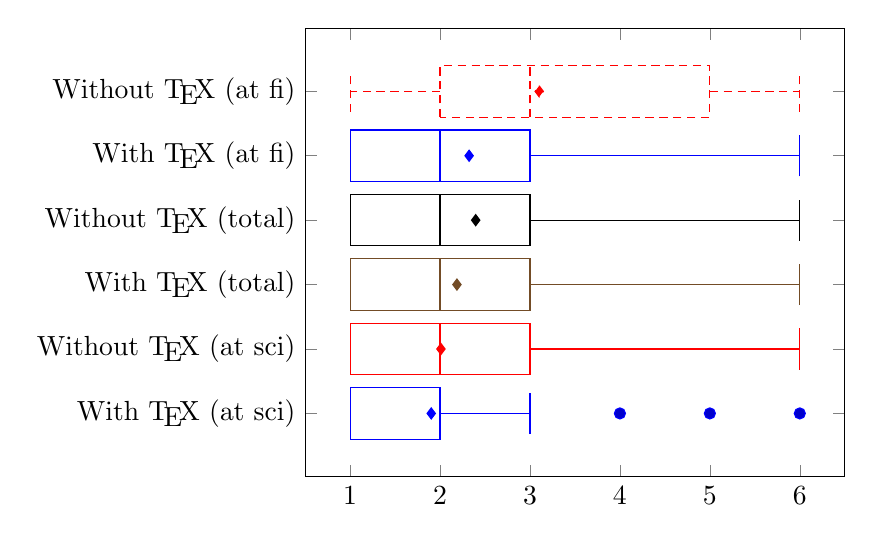
\begin{tikzpicture}
      \begin{axis}
        [
          ytick={1,2,3,4,5,6},
          yticklabels={With \TeX{} (at \acrshort{sci}),
                       Without \TeX{} (at \acrshort{sci}),
                       With \TeX{} (total),
                       Without \TeX{} (total),
                       With \TeX{} (at \acrshort{fi}),
                       Without \TeX{} (at \acrshort{fi})},
        ]
        \addplot+[
          boxplot prepared={
            upper quartile=2,
            median=1,
            lower quartile=1,
            upper whisker=3,
            lower whisker=1,
            average=1.90203562340967
          },
        ] table[row sep=\\,y index=0] {
          data\\ 4\\ 5\\ 6\\
        };
        \addplot+[
          boxplot prepared={
            upper quartile=3,
            median=2,
            lower quartile=1,
            upper whisker=6,
            lower whisker=1,
            average=2.01024727110715
          },
        ] table[row sep=\\,y index=0] {
          data\\
        };
        \addplot+[
          boxplot prepared={
            upper quartile=3,
            median=2,
            lower quartile=1,
            upper whisker=6,
            lower whisker=1,
            average=2.18796433878158
          },
        ] table[row sep=\\,y index=0] {
          data\\
        };
        \addplot+[
          boxplot prepared={
            upper quartile=3,
            median=2,
            lower quartile=1,
            upper whisker=6,
            lower whisker=1,
            average=2.39634545284606
          },
        ] table[row sep=\\,y index=0] {
          data\\
        };
        \addplot+[
          boxplot prepared={
            upper quartile=3,
            median=2,
            lower quartile=1,
            upper whisker=6,
            lower whisker=1,
            average=2.32342657342657
          },
        ] table[row sep=\\,y index=0] {
          data\\
        };
        \addplot+[
          boxplot prepared={
            upper quartile=5,
            median=3,
            lower quartile=2,
            upper whisker=6,
            lower whisker=1,
            average=3.1026936026936
          },
        ] table[row sep=\\,y index=0] {
          data\\
        };
      \end{axis}
    \end{tikzpicture}
    \caption{A box plot of the marks of theses written and defended between 2010 and 2015 at \gls{fi} and \gls{sci} with and without \gls{tex}}
    \label{fig:statistics-marks}
  \end{figure}

  A weak negative correlation ($R=-0.033$) was also found between the use of \gls{tex} and the marks given to theses defended between 2010 and 2015 at \gls{fi}. The author had therefore decided to test the following \gls{hypothesis}: Suppose the marks given to theses written and defended between 2010 and 2015 at \gls{mu} are normally distributed. Suppose also that the marks given to theses written using \gls{tex} have the expected value $\mu_1$ and the variance $\sigma_1^2$ and that the marks given to theses not written using \gls{tex} have the expected value $\mu_2$ and the variance $\sigma_2^2$. Under investigation is the \gls{hypothesis} that $\mu_1-\mu_2=0$ on the significance level $\alpha=0.01$. As an intermediary step, the $F$-test was used to test the \gls{hypothesis} that $\sigma_1^2/\sigma_2^2=1$ on the significance level $0.01$. Depending on the result, either the standard or Welsh's two-tailed unpaired two-sample $t$-test was used to test the original \gls{hypothesis}. As detailed in the table \ref{table:statistics-tex-marks}, I overall reject this \gls{hypothesis} on the significance level $0.01$. A box plot of the marks given to theses written and defended between 2010 and 2015 at \gls{fi} and \gls{sci} using and not using \gls{tex} is shown in the figure \ref{fig:statistics-marks}.

  \section{Comparison with Existing Solutions}
  As a part of the initial research, I also assessed several templates for the typesetting of theses in order to gather ideas for immediate and future improvements of the fithesis2 class. Initially, I'm going to focus on templates used at czech technical universities. I will then broaden the scope to include both the templates of foreign universities and other generic thesis typesetting \glspl{docclass}.

    \subsection{CTUStyle\index{CTUStyle|(} and CUStyle\index{CUStyle|(}}\label{sec:ctu&custyle}
    The first of the reviewed thesis typesetting templates were CTUStyle \cite{ctustyle} and CUStyle \cite{custyle} \glspl{texpackage} from RNDr. Petr Olšák, which were designed to be used at \gls{fel} and at \gls{cuni}, respectively. The sole dependencies of these templates are the \inx{\gls{csplain}} and \inx{\gls{opmac}} \glspl{texpackage}.

    The templates are closely tied with the visual styles of the universities, which is mainly achieved through color-coding. Aside from black-and-white text, the CTUstyle \gls{texpackage} typesets various typographic elements in the \clrpicker{pantone300} Pantone 300 color, which makes for a visually pleasing combination. The CUstyle \gls{texpackage} uses the combination of black, gray and \clrpicker{cured} Pantone 1797 color to a similar end. By typesetting various typographic elements in the \clrpicker{pantone122} Pantone 122 color, which is a part of the visual identity of \gls{fi} \cite{filogo}, and by replacing the logotype of the faculty with its colored version, which was created as a part of Matúš Kominka's bachelor thesis \cite{Kominka08}, the fithesis2 \gls{docclass} could be likewise revitalized. \partimp{v0.3.00, 01, 06} \pending{Color \cs{tt} and section names. Define and document \cs{facultyheadings}, \cs{facultyhyperlinks}, \cs{facultytables-light} and \cs{facultytables-dark} macros expanding to the names of colors of the given typographic elements.} Since each faculty of \gls{mu} has a color version of its logo \cite{muvis}, this redesign could be implemented without the loss of support for other faculties. \implemented{The logos were downloaded as monochromatic and direct color \gls{eps} files from \cite{muvis} and then transformed into \gls{pdf} files using the \texttt{epstopdf} \cite{epstopdf} utility.}

    Unlike with fithesis2, documents typeset with the CTUStyle and CUStyle templates are double-sided by default. The \gls{textwidth} of CTUStyle \eqref{eq:ctustyle-textwidth} and CUStyle \eqref{eq:custyle-textwidth}\begin{align}
      \label{eq:ctustyle-textwidth} 210\text{\,mm} \text{ (A4 width) } &- 2\cdot32\text{\,mm} \text{ \cite[line~249]{ctustyleCode} } &= 146\text{\,mm} \\
      \label{eq:custyle-textwidth}  210\text{\,mm} \text{ (A4 width) } &- 2\cdot31\text{\,mm} \text{ \cite[line~229]{custyleCode} } &= 148\text{\,mm}
    \end{align} is also much larger than that of fithesis2 (127\,mm \cite[lines~989, 1017, 1045]{fithesis2Code}). The margins of CTUStyle and CUStyle, in conjunction with the chosen font family, \label{overlong-lines} allow for up to 100 characters per line, which is not only wearying to the eye of an inexperienced reader \cite[section~2.1.2]{eletypostyle}, but also against the recommendations of \gls{fi} \cite[section~3.2.3]{bpdpfi}. As stated by the author of the styles \cite[post~25]{ctustyle-forums}, both decisions have likely been made in order to reduce the required storage space for the archival of physical prints of theses. \pending{Decrease the horizontal margins of fithesis3 loaded with the \texttt{twocolumn} option to achieve roughly 65 characters per line in each column with either the 11\,pt or the 10\,pt font size to make multicolumn typesetting viable. This would allow for more economical use of paper.}
    \index{CTUStyle|)}
    \index{CUStyle|)}

    \subsection{Felthesis\index{felthesis}}\label{sec:felthesis}
    Being a traditional \gls{docclass}, felthesis from Ing. Vít Zýka Ph. D. provides an alternative for those \gls{fel} students, who prefer \gls{latex} over \gls{csplain} used by the CTUStyle \gls{texpackage}. Much like fithesis1 and fithesis2, felthesis loads the KOMA-Script scrreprt \gls{docclass}, redefines some of the commands and \glspl{env}, loads additional packages and defines additional thesis sectioning commands. Unlike fithesis1 and fithesis2, felthesis loads babel and then selects the language based on the chosen language of the thesis \cite[lines~687--691]{felthesisCode} \pending{Load babel or polyglossia by default and pick the language based on \cs{@thesislang}}. Felthesis also loads biblatex \pending{} \cite[line~722]{felthesisCode}, automatically generates index \pending{} \cite[line~763]{felthesisCode} and stamps the title, author, subject, and keywords into the header of the resulting \gls{pdf} file \cite[lines~959--971]{felthesisCode} \label{pdf-stamping} \partimp{v0.3.02} \pending{Turn the \cs{ThesisKeyWords} \gls{env} into a command. Add a command or additional argument to provide keywords in English. These will be both typeset and stamped into the header of the resulting \gls{pdf} file.}. Alongside the package \gls{ltxpackage}, both a technical \cite{felthesisCode} and a user documentation \cite{felthesis} is distributed \pending{}.

    \subsection{The Charles University in Prague}
    Along with Petr Olšák's CUStyle, \gls{cuni} also provides an official \gls{latex} template for the typesetting of theses \cite{cunisablona}. Rather than defining a new \gls{docclass}, the archive contains a \gls{makefile} and a skeleton \gls{latex} document using the base report \gls{docclass} for both czech and english theses. The students then modify said document to suit their requirements. The template uses \gls{cslatex} rather than the babel \gls{ltxpackage}, which means that \gls{csfonts} rather than the superior \gls{lmfonts} \cite{cslatexvsbabel} are used by default.

    \subsection{Mendel University in Brno}\index{\texttt{dipp.sty}|(}\label{sec:dipp.sty}
    Despite not being an official thesis template of \gls{mendelu}, \texttt{dipp.sty} from doc. Ing. Dr. Jiří Rybička \gls{ltxpackage} warrants a mention. The package depends on the extended macro set of the \Hologo{XeTeX} \glslink{texeng}{typesetting engine} and is intended to be used with the base article \gls{docclass}. Although the article class was not designed with European typography in mind, the \texttt{dipp.sty} package redefines much of the geometry.

    Noteworthy is also the rich selection of additional markup, which is meant to ease the task of typesetting a thesis for those unfamiliar with \gls{latex}. To this end, thesis sectioning commands, macros and wrapper \glspl{env} for the inclusion of bibliography, tables or figures and discretionary macros specific to Czech typography such as \cs{az} for the typesetting of ranges and \cs{spoj} for hyphenation \cite{dippman}.\index{\texttt{dipp.sty}|)}

    \subsection{Brno University of Technology}\index{\texttt{thesis.sty}|(}
    The official thesis typesetting template of \gls{vut} is the \gls{ltxpackage} \texttt{thesis.sty}. Unlike \texttt{\hyperref[sec:dipp.sty]{\tt dipp.sty}}, \texttt{thesis.sty} is meant to be used with the base report \gls{docclass}. All packages required by the \gls{ltxpackage} are documented within \cite[p.~9]{thesis.sty-doc} \pending{}. The implicit \gls{textwidth} of the \gls{ltxpackage} is 150\,mm \cite[p.~2]{thesis.sty-doc}, which, in conjunction with the usage of \gls{csfonts} at 12\,pt, allows for up to 90 characters per line. This is problematic for reasons mentioned in section \ref{overlong-lines}.
    
    The \texttt{thesis.sty} \gls{ltxpackage} also adds provides additional markup. This includes wrapper commands such as \cs{novazkratka}, \cs{zk}, \cs{zkratka} and \cs{zkratkatext} for the typesetting of acronyms, the \cs{seznamzkratek} and \cs{literatura} \glspl{env} for acronyms and bibliography, respectively, and various math mode macros (see \cite[p.~6--9]{thesis.sty-doc}). Like \hyperref[sec:felthesis]{felthesis}, \texttt{thesis.sty} is also able to stamp thesis metadata into the \gls{pdf} header. The \texttt{thesis.sty} \gls{ltxpackage} can be downloaded from \cite{thesis.sty}.
    \index{\texttt{thesis.sty}|)}

    \subsection{Technical University of Liberec}\index{tul|(}\index{tulthesis|(}
    Unlike the preceding typesetting templates, tulthesis from doc. RNDr. Pavel Satrapa, Ph.D. is not a standalone \gls{docclass}, but rather a part of the tul \gls{ltxpackage}, which is the official \gls{ltxpackage} used for the typesetting of documents on \gls{tul}. The tulthesis \gls{docclass} uses the base report \gls{docclass} \cite[section~1]{tulthesis-man} and it is very visually distinctive. It inspired \cite[post~21]{ctustyle-forums} the creation of Petr Olšák's \nameref{sec:ctu&custyle} \glspl{texpackage}. The tul \gls{ltxpackage}, along with the tulthesis \gls{docclass}, can be downloaded from \cite{tul}.
    \index{tul|)}\index{tulthesis|)}

    \subsection{Techinal University of Ostrava}\index{diploma|(}
    The official style of \gls{vsb} is the diploma \gls{docclass} by Jiří Dvorský. Like Jiří Rybička's \hyperref[sec:dipp.sty]{\tt dipp.sty}, diploma uses the base article \gls{docclass}, modifies its geometry and adds thesis sectioning commands and additional macros for the users' convenience \cite{diploma}. The output documents are one-sided by default and the font size of 11\,pt is too small for the \gls{textwidth} of \begin{equation}
      \begin{split}
        210\,\text{mm} \text{ (A4 width) } &- 28\,\text{mm} \text{ (left margin) }  \\
                                           &- 32\,\text{mm} \text{ (right margin) }
                                            = 150\,\text{mm}
      \end{split}
    \end{equation} as defined in \cite[lines~111,~123]{diplomaSource}, resulting in overlong lines as discussed earlier (see section \ref{overlong-lines}).

    The additional macros range from mathematical \glspl{env} \cite[section~3.5]{diploma} and commands and \glspl{env} for the typesetting of code with syntax highlighting \cite[section~3.6]{diploma} \pending{} through commands for the insertion of graphics \cite[section~3.7]{diploma}.
    \index{diploma|)}

    \subsection{Silesian University in Opava}
    At the time of writing this thesis, there is no official or unofficial \gls{gls-docclass} or \gls{ltxpackage} of \gls{slu} available on the internet. There is a mention \cite{vavreckova} of the works on a \gls{docclass} at the webpage of RNDr. Šárka Vavřečková, Ph.D. who teaches typography at \acrlong{fpf}. There is also a bachelor's thesis \cite{hanzal09} written by Michal Hanzal from \gls{opf}. The author of the thesis describes the process of creating a \gls{gls-docclass} for what is supposed to be the official thesis typesetting template at \gls{opf}, but there is no mention of the style at the website of the faculty \cite{opftemplates}, although the linked dean's directives were written with \gls{latex} in mind.

    \subsection{Palacký Univerzity Olomouc}
    There are three independant \gls{latex} thesis typesetting templates available at \acrlong{upolsci} for the students at the departments of Experimental Physics, Informatics and Mathematical Analysis and Applications, respectively.

    The template used at the department of Experimental Physics is neither a \gls{docclass} nor a \gls{ltxpackage}. All definitions and alterations to the used built-it article \gls{docclass} are stored directly inside the example \gls{latex} source code, which the students are supposed to edit according to the needs of their theses. The template is supposed to be typeset using \glslink{cslatex}{\pdfCSLaTeX{}} \gls{texeng} meaning that \gls{csfonts} instead of the superior \gls{lmfonts} are used. Along with the thesis template, a \gls{beamer} template for thesis defense presentations is also distributed \pending{}. Both templates can be downloaded at \cite{upol-exfyz-template}.

    \index{KIdiplom|(} The template used at the department of Informatics is KIdiplom from Jan Outrata and Martin Rotter and it is a combination of a \gls{docclass}, which is based on the base article \gls{docclass} and is meant for the typesetting of theses, and a \gls{ltxpackage}, which was designed as a general \gls{ltxpackage} for the typesetting of documents in the visual style of the department of Informatics. Amongst the vices of the template are the disabled double-sided typing \cite[lines~69--72]{upol-inf-templateSource} and the \gls{textwidth} of\begin{equation}
    426\text{\,pt}\text{ (\texttt{a4paper} \gls{textwidth}) }\cdot1{,}05\text{ \cite[line~81]{upol-inf-templateSource} }\approx157,23\text{\,mm}
  \end{equation} in conjunction with the 12\,pt \gls{lmfonts} is too generous \cite[lines~74--82]{upol-inf-templateSource} causing overlong lines (see section \ref{overlong-lines}). The template by default loads \gls{biblatex} and \glspl{ltxpackage} for the typesetting of glossaries and index. The added convenience macros then comprise thesis sectioning commands and \glspl{env} for the typesetting of mathematical definitions, theorems or proofs and code snippets. Along with the thesis template, \gls{latex} templates for the typesetting of thesis reader's reports \pending{See the templates by \MR} and \gls{biblatex} ISO\hyph{}690 \cite{iso690-1,iso690-2} citation styles \pending{} are distributed. The templates can be downloaded at \cite{upol-inf-template}.\index{KIdiplom|)}
    
  \index{\texttt{maam-dipl.sty}|(}The template used at the department of Mathematical Analysis and Applications is a simple \gls{ltxpackage} \texttt{maam-dipl.sty}, which only defines basic thesis sectioning commands and is meant to be used with the base article \gls{docclass}. The template can be downloaded at \cite{upol-maam-template}\index{\texttt{maam-dipl.sty}|)}.

    % CTAN: http://www.ctan.org/topic/dissertation
    % Kumar07, https://tug.org/pracjourn/2007-4/


% \chapter{Results}
  \blindtext

  \section{\emph{Fithesis2} Class Improvements}  
  \blindtext

    \subsection{\Hologo{XeLaTeX} Engine Support} 
    \blindtext

    \subsection{OpenType Font Support} 
    \blindtext

  \section{Thesis Writing Guidelines} 
  \blindtext
% \chapter{Conclusions} 
  \blindtext

  % Bibliography
  \newpage
  \nocite{*}
  \tolerance=300
  \emergencystretch=1em
  \printbibliography[heading=bibintoc]
  \par

  % Glossary
  \newpage
  \printglossaries

  % Index
  \printindex

% \begin{appendices}
%   \chapter{Example Theses} 
  \blindtext
\chapter{User Guide} 
  \blindtext
\chapter{Technical Documentation} 
  \blindtext

% \end{appendices}

\end{document}
